\documentclass{article}

\usepackage{amsmath}
\usepackage{amssymb}
\usepackage{mathtools}
\usepackage{fullpage}
\usepackage[T1]{fontenc}
\usepackage{lmodern}
\usepackage{tikz}
\usetikzlibrary{calc,intersections,through,backgrounds}
\usetikzlibrary{bayesnet}
\usepackage{tikzscale}
\usepackage{tkz-euclide}
\usepackage{tcolorbox}
\tcbuselibrary{skins,breakable}
% pgfplots
\usepackage{pgfplots}
\pgfplotsset{compat=1.8}
% For entities in pgfplots
\newcommand{\entpgf}[1]{\texttt{#1}}

\begin{document}

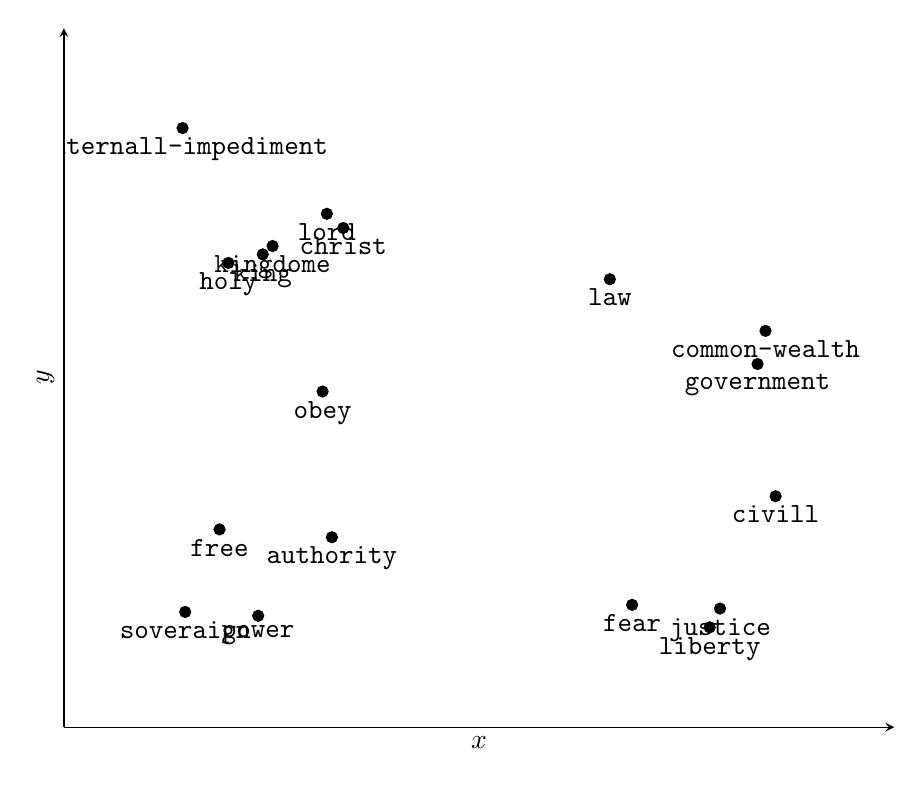
\begin{tikzpicture}
\pgfplotsset{ticks=none}
		\begin{axis}[
		    axis x line=bottom,
			axis y line=left,
			xmin=-39.91915-23.988705444335938, xmax=80.024376+23.988705444335938,
			ymin=-49.173088-24.026240539550784, ymax=70.958115+24.026240539550784,
			xtick={-39.91915,80.024376},ytick={-49.173088,70.958115},
			xlabel=$x$,ylabel=$y$,
			%x label style={anchor=west},
			%y label style={anchor=south},
			width=\textwidth
			]
			\addplot+[mark options={fill=black,color=black},only marks,point meta=explicit symbolic, nodes near coords] coordinates {
(46.503421783447266, 34.58695983886719)[]
(-24.62435531616211, -46.39107131958008)[]
(-39.39225387573242, -45.462982177734375)[]
(77.98419952392578, 22.16880226135254)[]
(-7.418119430541992, 46.909645080566406)[]
(-23.69881820678711, 40.56747817993164)[]
(80.02437591552734, -17.630285263061523)[]
(-9.717127799987793, -27.4947509765625)[]
(-21.712207794189453, 42.580501556396484)[]
(-11.602441787719727, 7.57306432723999)[]
(51.006492614746094, -43.76272964477539)[]
(-30.660472869873047, 38.5079345703125)[]
(76.3743896484375, 14.180973052978516)[]
(66.69720458984375, -49.17308807373047)[]
(-10.736512184143066, 50.325340270996094)[]
(68.78113555908203, -44.66043472290039)[]
(-32.444984436035156, -25.612884521484375)[]
(-39.919151306152344, 70.95811462402344)[]
};
\node (law) at (axis cs:46.50342, 34.58696){};
\node (power) at (axis cs:-24.624355, -46.39107){};
\node (soveraign) at (axis cs:-39.392254, -45.462982){};
\node (common-wealth) at (axis cs:77.9842, 22.168802){};
\node (christ) at (axis cs:-7.4181194, 46.909645){};
\node (king) at (axis cs:-23.698818, 40.56748){};
\node (civill) at (axis cs:80.024376, -17.630285){};
\node (authority) at (axis cs:-9.717128, -27.494751){};
\node (kingdome) at (axis cs:-21.712208, 42.5805){};
\node (obey) at (axis cs:-11.602442, 7.5730643){};
\node (fear) at (axis cs:51.006493, -43.76273){};
\node (holy) at (axis cs:-30.660473, 38.507935){};
\node (government) at (axis cs:76.37439, 14.180973){};
\node (liberty) at (axis cs:66.697205, -49.173088){};
\node (lord) at (axis cs:-10.736512, 50.32534){};
\node (justice) at (axis cs:68.781136, -44.660435){};
\node (free) at (axis cs:-32.444984, -25.612885){};
\node (externall-impediment) at (axis cs:-39.91915, 70.958115){};
\node[anchor = north, xshift=0.0, yshift=0.0] (lawl) at(axis cs: 46.50342, 34.58696){$\entpgf{law}$};
\node[anchor = north, xshift=0.0, yshift=0.0] (powerl) at(axis cs: -24.624355, -46.39107){$\entpgf{power}$};
\node[anchor = north, xshift=0.0, yshift=0.0] (soveraignl) at(axis cs: -39.392254, -45.462982){$\entpgf{soveraign}$};
\node[anchor = north, xshift=0.0, yshift=0.0] (common-wealthl) at(axis cs: 77.9842, 22.168802){$\entpgf{common-wealth}$};
\node[anchor = north, xshift=0.0, yshift=0.0] (christl) at(axis cs: -7.4181194, 46.909645){$\entpgf{christ}$};
\node[anchor = north, xshift=0.0, yshift=0.0] (kingl) at(axis cs: -23.698818, 40.56748){$\entpgf{king}$};
\node[anchor = north, xshift=0.0, yshift=0.0] (civilll) at(axis cs: 80.024376, -17.630285){$\entpgf{civill}$};
\node[anchor = north, xshift=0.0, yshift=0.0] (authorityl) at(axis cs: -9.717128, -27.494751){$\entpgf{authority}$};
\node[anchor = north, xshift=0.0, yshift=0.0] (kingdomel) at(axis cs: -21.712208, 42.5805){$\entpgf{kingdome}$};
\node[anchor = north, xshift=0.0, yshift=0.0] (obeyl) at(axis cs: -11.602442, 7.5730643){$\entpgf{obey}$};
\node[anchor = north, xshift=0.0, yshift=0.0] (fearl) at(axis cs: 51.006493, -43.76273){$\entpgf{fear}$};
\node[anchor = north, xshift=0.0, yshift=0.0] (holyl) at(axis cs: -30.660473, 38.507935){$\entpgf{holy}$};
\node[anchor = north, xshift=0.0, yshift=0.0] (governmentl) at(axis cs: 76.37439, 14.180973){$\entpgf{government}$};
\node[anchor = north, xshift=0.0, yshift=0.0] (libertyl) at(axis cs: 66.697205, -49.173088){$\entpgf{liberty}$};
\node[anchor = north, xshift=0.0, yshift=0.0] (lordl) at(axis cs: -10.736512, 50.32534){$\entpgf{lord}$};
\node[anchor = north, xshift=0.0, yshift=0.0] (justicel) at(axis cs: 68.781136, -44.660435){$\entpgf{justice}$};
\node[anchor = north, xshift=0.0, yshift=0.0] (freel) at(axis cs: -32.444984, -25.612885){$\entpgf{free}$};
\node[anchor = north, xshift=0.0, yshift=0.0] (externall-impedimentl) at(axis cs: -39.91915, 70.958115){$\entpgf{externall-impediment}$};

\end{axis}
\end{tikzpicture}

\end{document}